\documentclass[tikz,border=10pt]{standalone}
\usepackage{tikz}
\usetikzlibrary{arrows.meta,positioning,shapes,calc}

\begin{document}
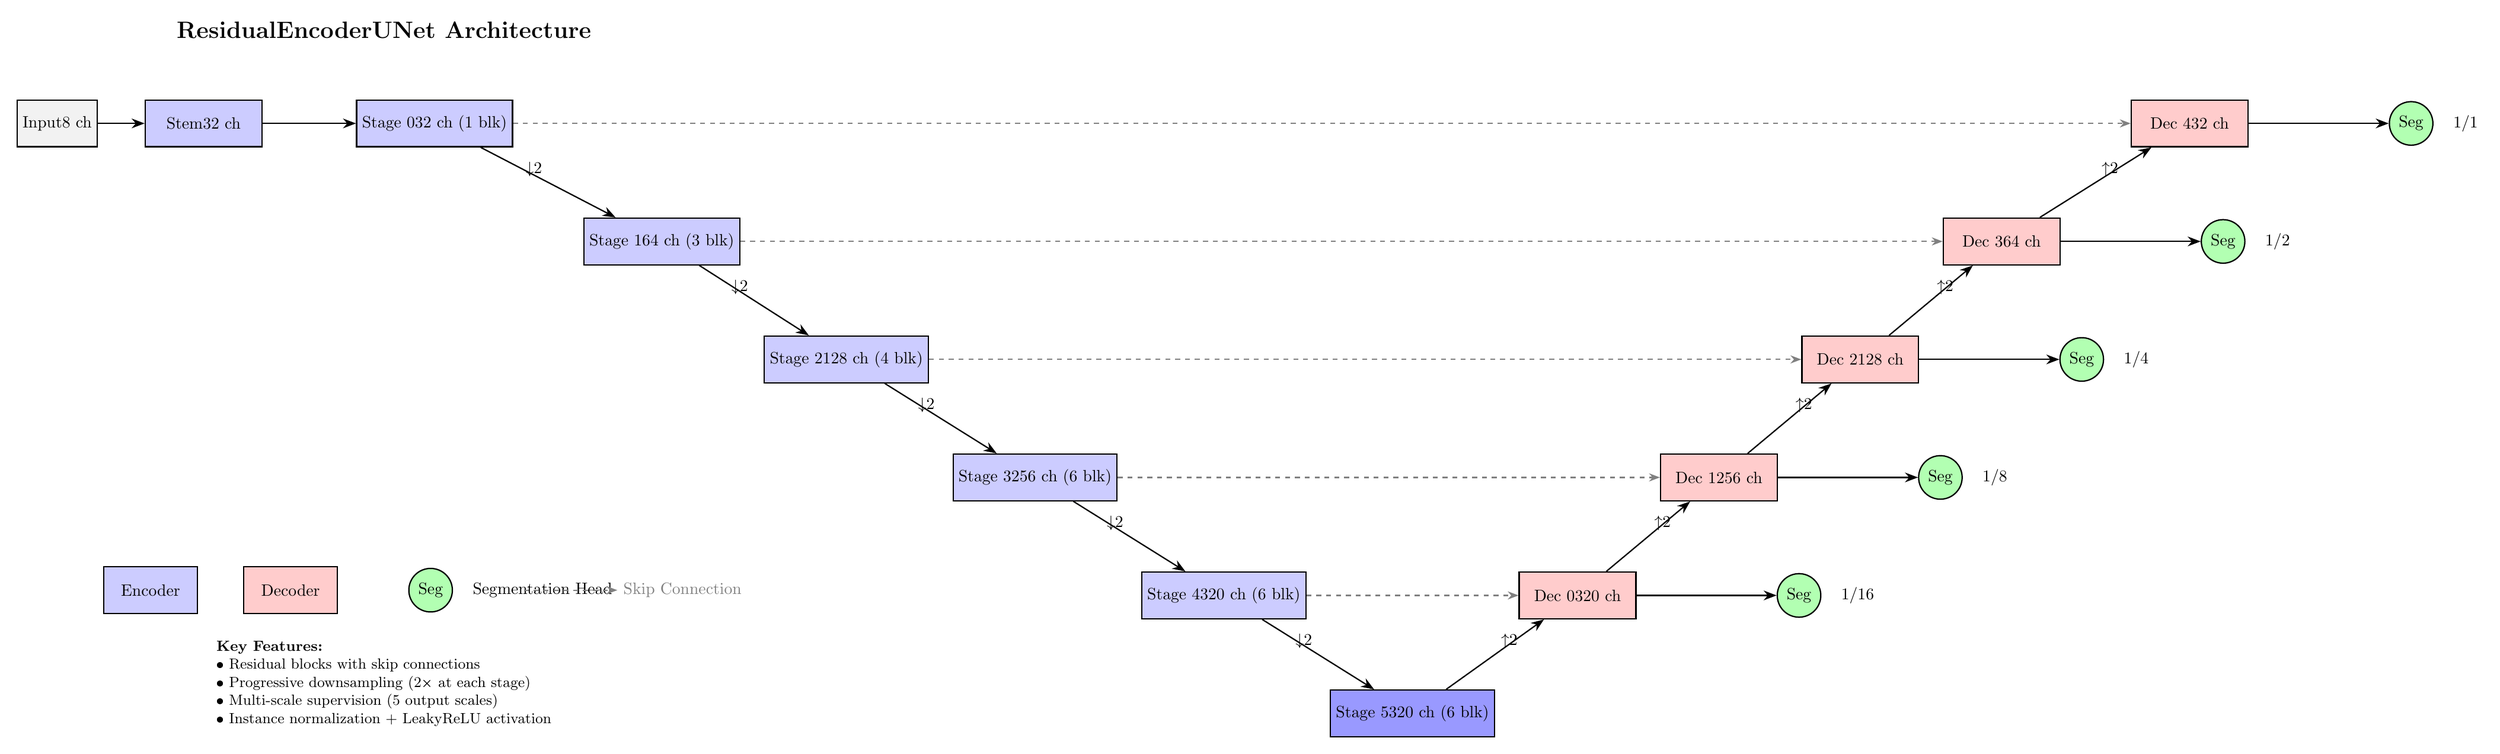
\begin{tikzpicture}[
    % Define styles
    encoder/.style={rectangle, draw, thick, fill=blue!20, minimum width=2.5cm, minimum height=1cm},
    decoder/.style={rectangle, draw, thick, fill=red!20, minimum width=2.5cm, minimum height=1cm},
    input/.style={rectangle, draw, thick, fill=gray!10, minimum width=1.5cm, minimum height=1cm},
    seg/.style={circle, draw, thick, fill=green!30, minimum size=0.8cm},
    arrow/.style={-{Stealth[scale=1.2]}, thick},
    skip/.style={dashed, thick, gray, -{Stealth[scale=1]}},
    node distance=1.5cm and 2cm
]

% Title
\node[font=\Large\bfseries] at (7,2) {ResidualEncoderUNet Architecture};

% Input
\node[input] (input) at (0,0) {Input\\8 ch};

% Encoder path
\node[encoder, right=1cm of input] (stem) {Stem\\32 ch};
\node[encoder, right=of stem] (stage0) {Stage 0\\32 ch (1 blk)};
\node[encoder, below right=1.5cm and 1.5cm of stage0] (stage1) {Stage 1\\64 ch (3 blk)};
\node[encoder, below right=1.5cm and 0.5cm of stage1] (stage2) {Stage 2\\128 ch (4 blk)};
\node[encoder, below right=1.5cm and 0.5cm of stage2] (stage3) {Stage 3\\256 ch (6 blk)};
\node[encoder, below right=1.5cm and 0.5cm of stage3] (stage4) {Stage 4\\320 ch (6 blk)};
\node[encoder, below right=1.5cm and 0.5cm of stage4, fill=blue!40] (stage5) {Stage 5\\320 ch (6 blk)};

% Decoder path
\node[decoder, above right=1.5cm and 0.5cm of stage5] (dec0) {Dec 0\\320 ch};
\node[decoder, above right=1.5cm and 0.5cm of dec0] (dec1) {Dec 1\\256 ch};
\node[decoder, above right=1.5cm and 0.5cm of dec1] (dec2) {Dec 2\\128 ch};
\node[decoder, above right=1.5cm and 0.5cm of dec2] (dec3) {Dec 3\\64 ch};
\node[decoder, above right=1.5cm and 1.5cm of dec3] (dec4) {Dec 4\\32 ch};

% Segmentation heads
\node[seg, right=3cm of dec0] (seg0) {Seg};
\node[seg, right=3cm of dec1] (seg1) {Seg};
\node[seg, right=3cm of dec2] (seg2) {Seg};
\node[seg, right=3cm of dec3] (seg3) {Seg};
\node[seg, right=3cm of dec4] (seg4) {Seg};

% Resolution labels
\node[right=0.3cm of seg0] {1/16};
\node[right=0.3cm of seg1] {1/8};
\node[right=0.3cm of seg2] {1/4};
\node[right=0.3cm of seg3] {1/2};
\node[right=0.3cm of seg4] {1/1};

% Encoder connections
\draw[arrow] (input) -- (stem);
\draw[arrow] (stem) -- (stage0);
\draw[arrow] (stage0) -- (stage1) node[midway, above left] {$\downarrow$2};
\draw[arrow] (stage1) -- (stage2) node[midway, above left] {$\downarrow$2};
\draw[arrow] (stage2) -- (stage3) node[midway, above left] {$\downarrow$2};
\draw[arrow] (stage3) -- (stage4) node[midway, above left] {$\downarrow$2};
\draw[arrow] (stage4) -- (stage5) node[midway, above left] {$\downarrow$2};

% Decoder connections
\draw[arrow] (stage5) -- (dec0) node[midway, above right] {$\uparrow$2};
\draw[arrow] (dec0) -- (dec1) node[midway, above right] {$\uparrow$2};
\draw[arrow] (dec1) -- (dec2) node[midway, above right] {$\uparrow$2};
\draw[arrow] (dec2) -- (dec3) node[midway, above right] {$\uparrow$2};
\draw[arrow] (dec3) -- (dec4) node[midway, above right] {$\uparrow$2};

% Skip connections
\draw[skip] (stage4.east) -- (dec0.west);
\draw[skip] (stage3.east) -- (dec1.west);
\draw[skip] (stage2.east) -- (dec2.west);
\draw[skip] (stage1.east) -- (dec3.west);
\draw[skip] (stage0.east) -- (dec4.west);

% Connections to segmentation heads
\draw[arrow] (dec0) -- (seg0);
\draw[arrow] (dec1) -- (seg1);
\draw[arrow] (dec2) -- (seg2);
\draw[arrow] (dec3) -- (seg3);
\draw[arrow] (dec4) -- (seg4);

% Legend
\node[encoder, minimum width=2cm] at (2,-10) (leg_enc) {Encoder};
\node[decoder, minimum width=2cm] at (5,-10) (leg_dec) {Decoder};
\node[seg] at (8,-10) (leg_seg) {Seg};
\node[right=0.3cm of leg_seg] {Segmentation Head};
\draw[skip] (10,-10) -- (12,-10) node[right] {Skip Connection};

% Key features
\node[align=left, font=\small] at (7,-12) {
    \textbf{Key Features:}\\
    • Residual blocks with skip connections\\
    • Progressive downsampling (2× at each stage)\\
    • Multi-scale supervision (5 output scales)\\
    • Instance normalization + LeakyReLU activation
};

\end{tikzpicture}
\end{document}